\subsection{MVC 模式}

MVC,即模型-视图-控制器,是一种用于构建图形用户界面应用程序的常用设计模式。它将应用程序分成三个独立的部分:模型、视图和控制器。

\begin{figure}[htb]
  \centering
  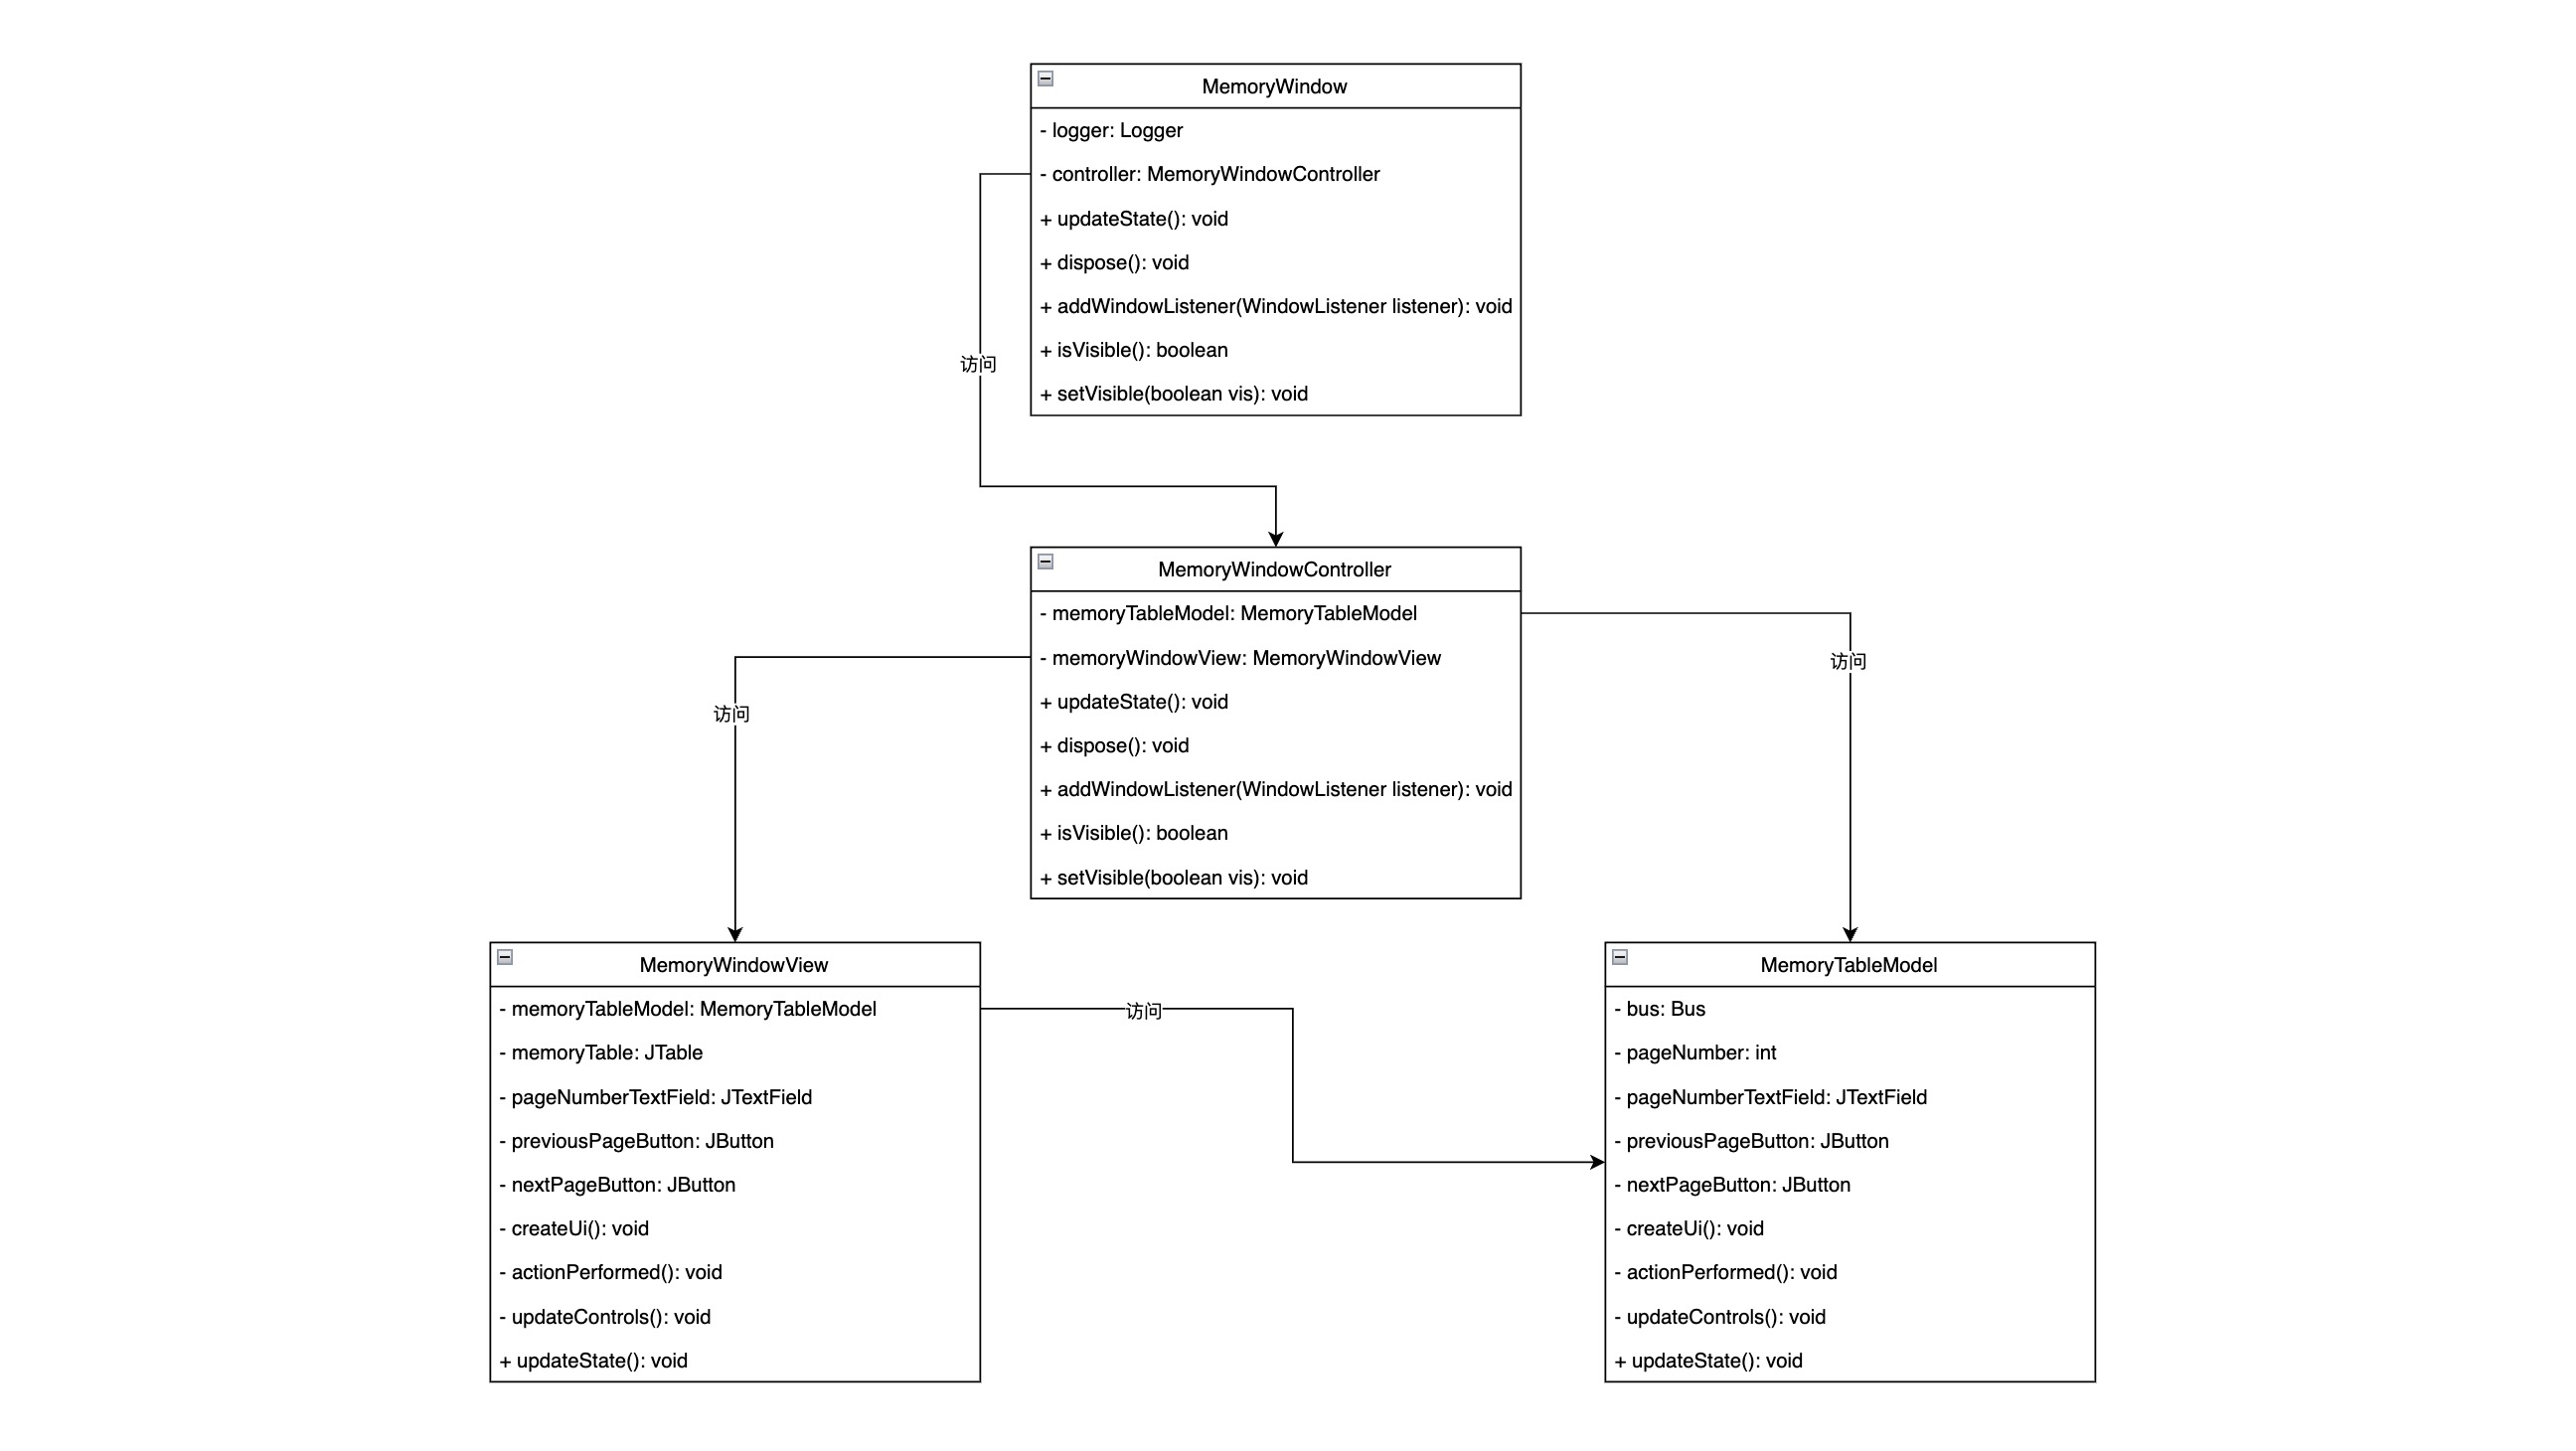
\includegraphics[width=0.9\textwidth]{figures/MVC模式.jpg}
  \caption{MVC 模式在 Slow6502 中的类图}
\end{figure}

在MemoryWindow页面使用MVC模式,使得逻辑控制、组件UI实现、数据模型处理逻辑分离,能够使得前端整体架构更加解耦。控制器的职责是接收用户的输入并将其转发给模型,然后根据模型的响应更新视图。

